\section{相对上同调}
\sourcepage{315--316}
继续讨论单纯上同调，定义相对群、单纯映射诱导的同态及长正合列。它们有些方面类似相对同调，有些方面却相当不同。

\entry{定义}{5.4.1}若 $K_0$ 为 $K$ 的子复形，则\textbf{相对上链群}为
\[
C^p(K,K_0;G)=\operatorname{Hom}(C_p(K,K_0),G).
\]
相对上边缘为相对边缘的对偶，记为 $\delta$。其核、像分别为相对上闭链群 $Z^p$、相对上边缘群 $B^{p+1}$，定义
\[
H^p(K,K_0;G)=Z^p(K,K_0;G)/B^p(K,K_0;G).
\]
相对上链的几何理解与相对链不同。链群短正合列
\[
0\to C_p(K_0)\xrightarrow{i}C_p(K)\xrightarrow{j}C_p(K,K_0)\to0
\]
因商群自由而分裂。对偶后仍为分裂短正合列
\[
0\leftarrow C^p(K_0;G)\xleftarrow{\overline i}C^p(K;G)
\xleftarrow{\overline j}C^p(K,K_0;G)\leftarrow0.
\]
于是，相对上链群自然是绝对上链群的\emph{子群}，而子复形的上链群自然是其\emph{商群}。

具体地，从商链群到 $G$ 的同态，恰对应于在 $C_p(K_0)$ 上为零的同态。因此可以把相对上链认同为在 $K_0$ 的每个有向单形上都为零的上链。某种意义上，它们由 $K\setminus K_0$ “承载”。这一子群被 $\delta$ 保持：若 $\tau$ 是 $K_0$ 的单形，则其边缘也在 $K_0$ 内，所以 $\langle\delta c^p,\tau\rangle=\langle c^p,\partial\tau\rangle=0$。

\sourcepage{317}
因此投影 $j$ 的对偶是包含映射，而包含 $i$ 的对偶是把上链限制到 $C_p(K_0)$ 的限制映射。

若 $f:(K,K_0)\to(L,L_0)$ 为单纯映射，其相对链映射 $f_\#$ 的对偶记为 $f^\#$。由 $f_\#\partial=\partial f_\#$，得 $\delta f^\#=f^\#\delta$。它称为\textbf{上链映射}（cochain map），将上闭链、上边缘分别映为上闭链、上边缘，诱导
\[
f^*:H^p(L,L_0;G)\to H^p(K,K_0;G).
\]
函子性质在上链层次已经成立：恒等映射诱导恒等，而 $(g\circ f)^\#=f^\#g^\#$。

\entry{定理}{5.4.2}存在长正合列
\[
\cdots\leftarrow H^p(K_0;G)\leftarrow H^p(K;G)\leftarrow H^p(K,K_0;G)
\xleftarrow{\delta^*}H^{p-1}(K_0;G)\leftarrow\cdots.
\]
若 $K_0\ne\varnothing$，约化上同调也有类似序列。单纯映射诱导相应长正合列之间的同态。

\sourcepage{318}
\textbf{证明：}将逐维分裂的上链短正合列与各 $\delta$ 排成交换图，应用之字形引理（引理 3.3.2）。虽然箭头方向与链复形相反，方法完全相同，连接同态 $\delta^*$ 使维数增加一维。

对约化情形，在零维下面补上短正合列 $0\leftarrow G\xleftarrow{\operatorname{id}}G\leftarrow0\leftarrow0$，并以余增广连接到零维上链列，即可作同样论证。余增广单射，所以负一维没有非零上同调。自然性也由之字形引理得到。\hfill$\square$

\entry{例}{5.4.3}取图 5.4.1 的正方形复形 $K$ 及其边界 $K_0$。相对上链就是在边界上为零的上链。二维相对上闭链由 $\sigma_1^*,\sigma_2^*$ 生成，一维相对上链由 $e_5^*$ 生成，且 $\delta e_5^*=\sigma_1^*-\sigma_2^*$。所以 $H^2(K,K_0)\cong\Z$，生成元为两者共同的上同调类。
\begin{center}
\includegraphics[width=.96\textwidth]{figures/5-4-1.pdf}\\图 5.4.1\end{center}
没有非零相对一维上闭链，也没有非零相对零维上链，故 $H^1(K,K_0)=H^0(K,K_0)=0$。

\sourcepage{319}
结合边界圆周的计算，长正合列的一段变为
\[
0\leftarrow H^2(K)\leftarrow\Z\xleftarrow{\delta^*}\Z\leftarrow H^1(K)\leftarrow0.
\]
还需计算连接同态。$H^1(K_0)$ 由 $e_1^*$ 的类生成。先将它延拓为 $K$ 上同名上链，再取上边缘，并视为相对上链，即得到 $\delta^*$。由 $\delta e_1^*=-\sigma_1^*$，可知连接同态为同构。因此两个未知群 $H^2(K),H^1(K)$ 都为零。

\entry{例}{5.4.4}考虑图 5.4.2 的 Möbius 带 $M$ 及其边界 $E$。计算空间偶与空间本身的上同调。
\begin{center}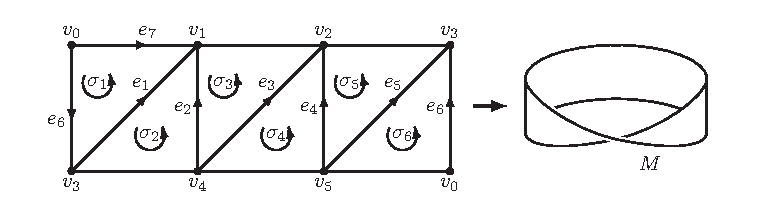
\includegraphics[width=.96\textwidth]{figures/5-4-2.pdf}\\图 5.4.2\end{center}
二维相对上闭链以六个 $\sigma_i^*$ 为基，一维相对上链以 $e_1^*,\ldots,e_6^*$ 为基。改用基
\[
\sigma_1^*,\ \sigma_1^*-\sigma_2^*,\ \ldots,\ \sigma_5^*-\sigma_6^*
\]
及
\[
e_1^*,\ldots,e_5^*,\ e_1^*+\cdots+e_6^*.
\]
有 $\delta e_i^*=\sigma_i^*-\sigma_{i+1}^*$（$1\le i\le5$），且最后一个基元的上边缘为 $2\sigma_1^*$。因此 $H^2(M,E)\cong\Z/2$，由 $\sigma_1^*$ 的类生成。上边缘把一维基映为一个子群的基，故一维核为零，$H^1(M,E)=0$；零维相对上链为零，故 $H^0(M,E)=0$。

\sourcepage{320}
边界 $E$ 是六边形，故 $H^1(E)\cong\Z$、$H^2(E)=0$。长正合列为
\[
0\leftarrow H^2(M)\leftarrow\Z/2\xleftarrow{\delta^*}\Z\leftarrow H^1(M)\leftarrow0.
\]
取边界边 $e_7$，其初等上链的类生成 $H^1(E)$。延拓后直接计算 $\delta e_7^*=-\sigma_1^*$，所以连接同态满射。由正合性，$H^2(M)=0$，$H^1(M)\cong\Z$。

下面定义以后会多次出现的伪流形。

\entry{定义}{5.4.5}若单纯偶 $(K,K_0)$ 满足下列条件，称为\textbf{相对 $n$ 维伪流形}（relative pseudo $n$-manifold）：
\begin{enumerate}[label=(\arabic*)]
\item $\overline{|K|\setminus|K_0|}$ 为一些 $n$ 维单形之并。
\item 每个不在 $K_0$ 中的 $(n-1)$ 维单形，恰为两个 $n$ 维单形的面。
\item 任意两个不在 $K_0$ 中的 $n$ 维单形 $\sigma,\sigma'$，都可由序列 $\sigma=\sigma_0,\ldots,\sigma_k=\sigma'$ 连接，其中各单形不在 $K_0$ 中，且每个相邻交都是不在 $K_0$ 中的 $(n-1)$ 维单形。
\end{enumerate}
若 $K_0=\varnothing$，称 $K$ 为 $n$ 维伪流形。

\sourcepage{321}
定义同调时，各单形的定向可以任意选择，彼此无须关联。但知道顶维单形能否协调定向，往往很有用。

\entry{定义}{5.4.6}在相对伪流形中，取两个不同顶维单形及上述无重复的连接序列（存在性见习题 5(a)）。一旦首个单形定向，就能唯一依次为其他单形定向，使 $\partial\sigma_{i-1}+\partial\sigma_i$ 在公共面上的系数为零。称末个单形的定向为沿此序列\textbf{诱导的定向}。

固定一个不在 $K_0$ 中的顶维单形及其定向。若它在每个其他顶维单形上诱导的定向都与连接序列无关，称 $(K,K_0)$ \textbf{可定向}（orientable）；否则称\textbf{不可定向}。

\subsection*{习题}
\begin{enumerate}
\item 对例 5.4.4 的 Möbius 带，找一个代表 $H^1(M)$ 生成元的上闭链。
\item 取圆柱面 $C$ 及一条边界圆周 $E$。
\begin{enumerate}[label=(\alph*)]
\item 计算 $H^i(C,E)$。
\item 用空间偶的长正合列计算 $H^i(C)$。
\end{enumerate}
\item 下列空间在通常三角剖分下，哪些是伪流形？
\begin{enumerate}[label=(\alph*)]
\item $S^1$；
\item $S^2$；
\item 字母 $\theta$ 形曲线；
\item $S^2$ 与一条仅与它交于一点的圆周之并；
\item 两个球面共用一点所得空间；
\item 把球面的南北极认同所得空间。
\end{enumerate}
\item 证明紧连通二维流形在通常三角剖分下是伪流形。〔以后会证明每个连通的三角剖分 $n$ 维流形都是 $n$ 维伪流形。〕\translatornote{原书此句省略了连通条件；由定义中的条件 (3)，不连通流形不满足所要求的伪流形定义。}
\item 设 $(K,K_0)$ 为相对 $n$ 维伪流形。
\begin{enumerate}[label=(\alph*)]
\item 证明任意两个不同的、均不在 $K_0$ 中的顶维单形，都有定义 5.4.5(3) 所要求的无重复连接序列。
\item 若 $K$ 有限，证明可定向时 $H_n(K,K_0)\cong\Z$、$H^n(K,K_0)\cong\Z$；不可定向时 $H_n(K,K_0)=0$、$H^n(K,K_0)\cong\Z/2$。〔提示：任意定向所有相对顶维单形并取和 $\gamma$，则对每个相对 $(n-1)$ 维上链，$\langle\delta c^{n-1},\gamma\rangle$ 为偶数。因此 $\sigma^*$ 不是上边缘。〕
\item 推出至少在有限情形，可定向性不依赖初始单形的选择，事实上只依赖拓扑空间偶，而不依赖具体三角剖分。
\item 有限情形下证明 $H_n(K,K_0;\Z/2)\cong\Z/2\cong H^n(K,K_0;\Z/2)$。
\end{enumerate}
\end{enumerate}
